
\begin{frame}{Motivation}

Inferring population structure from genomic sequences.
\begin{itemize}
  \item[--] Genetic data from Taita thrush, an endangered bird species native to Kenya
  {\color{blue} \href{https://web.stanford.edu/group/pritchardlab/publications/pdfs/PritchardEtAl00.pdf}{(Pritchard et al. 2011)}}.

  \item[--] Microsatellites sequences of 155 individiuals at 7 loci.
\end{itemize}


\begin{figure}[!h]
\centering
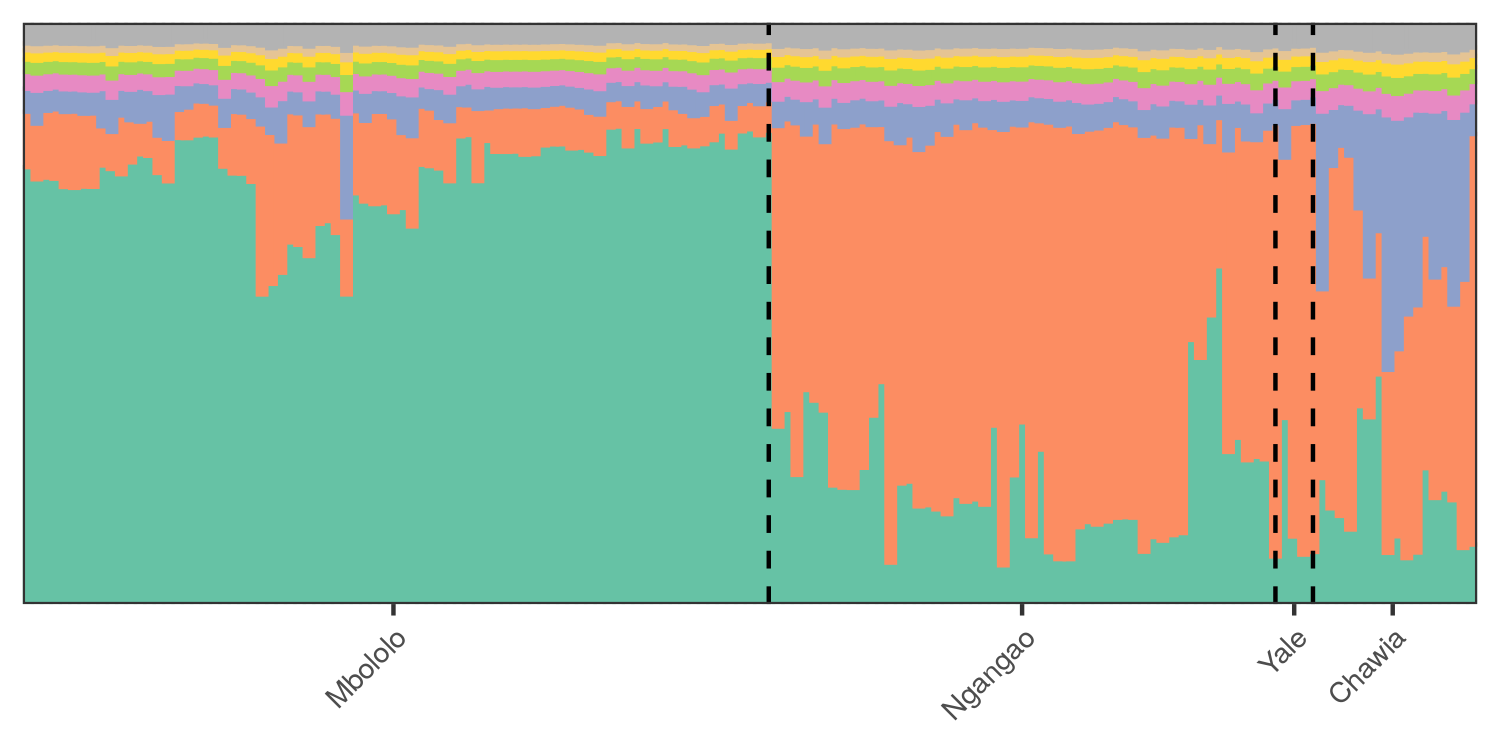
\includegraphics[width = 0.8\textwidth]{./figures/structure_example.png}
\end{figure}

\end{frame}

\begin{frame}{Motivation}

\begin{figure}[!h]
\centering
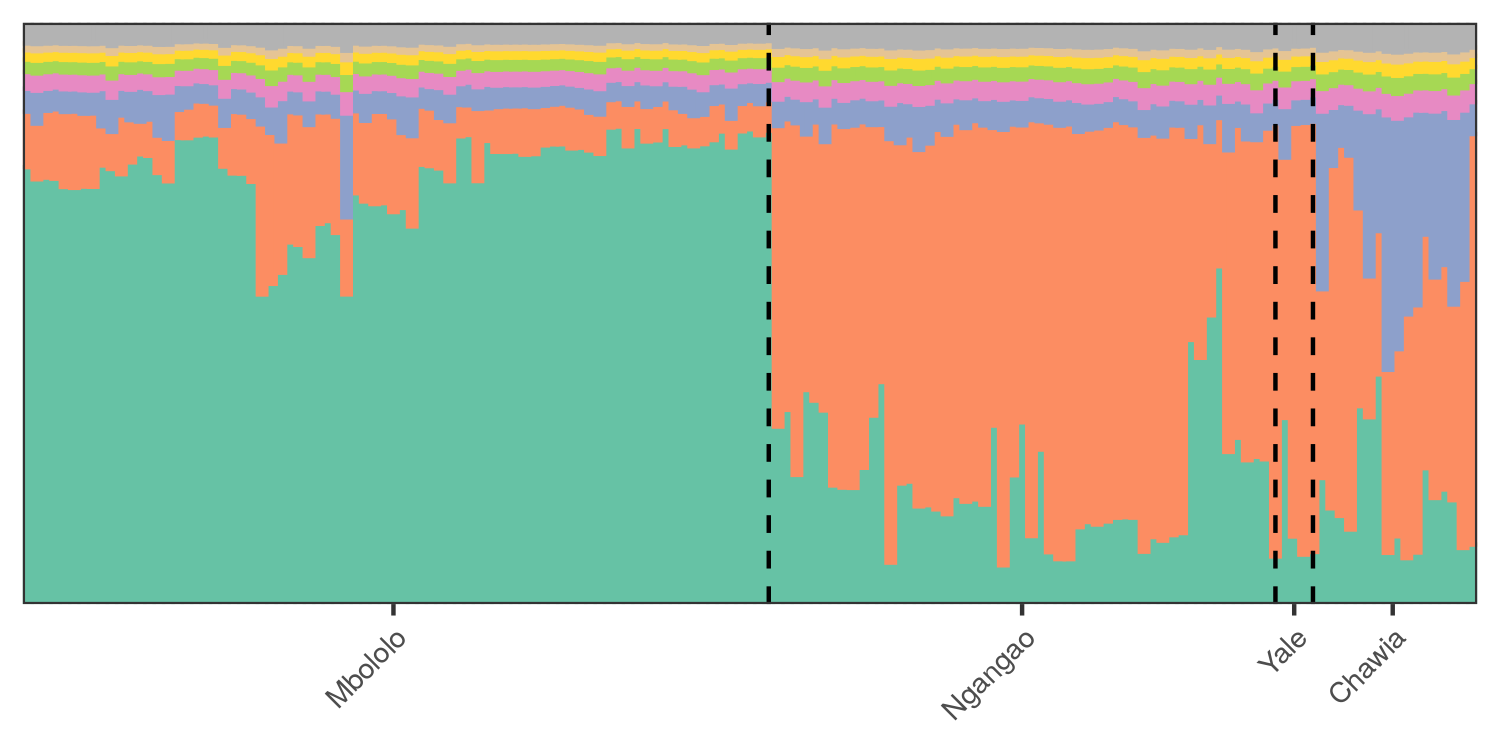
\includegraphics[width = 0.8\textwidth]{./figures/structure_example.png}
\end{figure}

\vspace{-1em}

{\bf Possible questions of interest: }

\begin{enumerate}
    \item How many latent populations---aka clusters---are present in the data set?
    \pause
    \item Which individuals cluster together?
    \pause
    \item What are the unique characterstics of each cluster?
\end{enumerate}


\end{frame}
\begin{frame}{Research problem}

A Bayesian nonparametric (BNP) model makes inferring the number of clusters amenable to
Bayesian inference.

\pause

We approximate the exact posterior using variational Bayes.

\pause

\textbf{Question}: how sensitive is the VB approximation, and the resulting
inferences, to BNP model choices?

\pause

\textbf{Problem}: re-running VB for multiple model choices is expensive.

\pause

\textbf{We propose}: a linear approximation to efficiently
estimate BNP sensitivity from a single run of VB (to avoid
expensive refitting).

\end{frame}

\begin{frame}{Outline}
\begin{itemize}
\item The BNP model
\vspace{0.1in}

\item The variational approximation
\vspace{0.1in}

\item Hyperparameter sensitivity
\vspace{0.1in}

\item Functional sensitivity and influence functions
\vspace{0.1in}

\item Results on population genetics modeling of the Taita thrush
\vspace{0.1in}

\end{itemize}
\end{frame}
